\documentclass{beamer}
\usecolortheme{dove}
\setbeamertemplate{navigation symbols}{}
\newenvironment{alltt}{\ttfamily}{\par}
\usepackage{amsmath,amssymb,amsfonts,amsthm, multicol, subfigure, color}
\usepackage{bm}
\usepackage{graphicx}
\usepackage{tabularx}
\usepackage{booktabs}
\usepackage{hyperref}
\usepackage{pdfpages}
\usepackage{xcolor}
\definecolor{dodgerblue}{rgb}{.118, .575, 1}
\definecolor{seagreen4}{RGB}{46, 139, 87}
\def\independenT#1#2{\mathrel{\rlap{$#1#2$}\mkern2mu{#1#2}}}
\newcommand\independent{\protect\mathpalette{\protect\independenT}{\perp}}
\newcommand\indep{\protect\mathpalette{\protect\independenT}{\perp}}
\def\logit{\text{logit}}
\usepackage{stackrel}
\usepackage{tikz}
\usetikzlibrary{arrows,shapes.arrows,positioning,shapes,patterns,calc}
\newcommand\slideref[1]{\vskip .1cm \scriptsize \textcolor{gray}{{#1}}}
\definecolor{seagreen}{RGB}{46, 139, 87}
\newcommand\red[1]{\color{red}#1}
\newcommand\blue[1]{\color{blue}#1}
\newcommand\gray[1]{\color{gray}#1}
\newcommand\green[1]{\color{olive}#1}
\newcommand\seagreen[1]{\color{seagreen}#1}
\newcommand\purple[1]{\color{purple}#1}
\newcommand\orange[1]{\color{orange}#1}
\newcommand\black[1]{\color{black}#1}
\newcommand\white[1]{\color{white}#1}
\newcommand\teal[1]{\color{teal}#1}
\newcommand\magenta[1]{\color{magenta}#1}
\newcommand\Fuchsia[1]{\color{Fuchsia}#1}
\newcommand\BlueGreen[1]{\color{BlueGreen}#1}
\newcommand\bblue[1]{\textcolor{blue}{\textbf{#1}}}
\newcommand\bred[1]{\textcolor{red}{\textbf{#1}}}
\newcommand\bgray[1]{\textcolor{gray}{\textbf{#1}}}
\newcommand\bgreen[1]{\textcolor{seagreen}{\textbf{#1}}}
\colorlet{lightgray}{gray!40}
\pgfdeclarelayer{bg}    % declare background layer for tikz
\pgfsetlayers{bg,main} % order layers for tikz
\newcommand\bref[2]{\href{#1}{\color{blue}{#2}}}
\newcommand\mycite[1]{\begin{scriptsize}\textcolor{darkgray}{(#1)}\end{scriptsize}}
\newcommand\iid{\stackrel{\text{iid}}{\sim}}
\newcommand\E{\text{E}}
\newcommand\V{\text{V}}
\renewcommand\P{\text{P}}
\newcommand{\Cov}{\text{Cov}}
\newcommand{\Cor}{\text{Cor}}
\newcommand\doop{\text{do}}
\newcommand{\tcframe}{\frame{
\small{
\only<1|handout:0>{\tableofcontents}
\only<2|handout:1>{\tableofcontents[currentsection]}}
}}
% Credit for the following to https://tex.stackexchange.com/questions/44983/beamer-removing-headline-and-its-space-on-a-single-frame-for-plan-but-keepin
\makeatletter
    \newenvironment{withoutheadline}{
        \setbeamertemplate{headline}[default]
        \def\beamer@entrycode{\vspace*{-\headheight}}
    }{}
\makeatother
\setbeamercovered{invisible}
\usepackage[round]{natbib}
\bibliographystyle{humannat-mod}
\setbeamertemplate{enumerate items}[default]
\usepackage{mathtools}
% BELOW THREE LINES MAKES NAME IN FOOTER
%\setbeamertemplate{footline}[text line]{%
%\parbox{\linewidth}{\vspace*{-8pt}Lundberg, Johnson, and Stewart. What is Your Estimand?}}%\hfill\insertshortauthor\hfill\insertpagenumber}}

%\setbeamertemplate{footline}[text line]{%
%\parbox{\linewidth}{\vspace*{-8pt}Ian Lundberg (Princeton)}}%\hfill\insertshortauthor\hfill\insertpagenumber}}
%t\setbeamertemplate{navigation symbols}{}

% Make the header figure that will appear frequently
\newcommand\headerfigure{
\begin{tikzpicture}[x = \textwidth, y = \textheight, every node/.style={anchor = center}]
\node at (0,1) {\resizebox{\textwidth}{!}{\begin{tikzpicture}[x = 1.7in, y = .3in]
    \node[cloud, draw, align=center, cloud puffs=20,cloud puff arc=110, aspect=2, inner sep=.5mm, font = \small] (general) at (-.1,0) {Theory or\\general goal};
    %%%%%%%%%%
    \node[align=center, font = \small] (theoretical) at (1,0) {Theoretical\\estimand};
    \draw[->, thick] (general) -- (theoretical);
    \node[align = center, anchor = south, font = {\bf\small}] at (.5,0) {Set};
    \node[align = center, anchor = north, font = \small] at (.5,0) {by argument};
    %%%%%%%%%%
    \node[align=center, font = \small] (empirical) at (2,0) {Empirical\\estimand};
    \draw[->, thick] (theoretical) -- (empirical);
    \node[align = center, anchor = south, font = {\bf\small}] at (1.5,0) {Link};
    \node[align = center, anchor = north, font = \small] at (1.5,0) {by assumption};
    %%%%%%%%%%
    \node[align=center, font = \small] (estimate) at (3,0) {Estimation\\strategy};
    \draw[->, thick] (empirical) -- (estimate);
    \node[align = center, anchor = south, font = {\bf\small}] at (2.5,0) {Learn};
    \node[align = center, anchor = north, font = \small] at (2.5,0) {by data};
    \end{tikzpicture}
    }};
\end{tikzpicture}
}
% Make the versions that have only one step in black
\newcommand\headerfigureset{
\begin{tikzpicture}[x = \textwidth, y = \textheight, every node/.style={anchor = center}]
\node at (0,1) {\resizebox{\textwidth}{!}{\begin{tikzpicture}[x = 1.7in, y = .3in]
    \node[cloud, draw, align=center, cloud puffs=20,cloud puff arc=110, aspect=2, inner sep=.5mm, font = \small] (general) at (-.1,0) {Theory or\\general goal};
    %%%%%%%%%%
    \node[align=center, font = \small] (theoretical) at (1,0) {Theoretical\\estimand};
    \draw[->, thick] (general) -- (theoretical);
    \node[align = center, anchor = south, font = {\bf\small}] at (.5,0) {Set};
    \node[align = center, anchor = north, font = \small] at (.5,0) {by argument};
    %%%%%%%%%%
    \node[align=center, font = \small, gray] (empirical) at (2,0) {Empirical\\estimand};
    \draw[->, thick, gray] (theoretical) -- (empirical);
    \node[align = center, anchor = south, font = {\bf\small}, gray] at (1.5,0) {Link};
    \node[align = center, anchor = north, font = \small, gray] at (1.5,0) {by assumption};
    %%%%%%%%%%
    \node[align=center, font = \small, gray] (estimate) at (3,0) {Estimation\\strategy};
    \draw[->, thick, gray] (empirical) -- (estimate);
    \node[align = center, anchor = south, font = {\bf\small}, gray] at (2.5,0) {Learn};
    \node[align = center, anchor = north, font = \small, gray] at (2.5,0) {by data};
    \end{tikzpicture}
    }};
\end{tikzpicture}
}
\newcommand\headerfigurelink{
\begin{tikzpicture}[x = \textwidth, y = \textheight, every node/.style={anchor = center}]
\node at (0,1) {\resizebox{\textwidth}{!}{\begin{tikzpicture}[x = 1.7in, y = .3in]
    \node[cloud, draw, align=center, cloud puffs=20,cloud puff arc=110, aspect=2, inner sep=.5mm, font = \small, gray] (general) at (-.1,0) {Theory or\\general goal};
    %%%%%%%%%%
    \node[align=center, font = \small] (theoretical) at (1,0) {Theoretical\\estimand};
    \draw[->, thick, gray] (general) -- (theoretical);
    \node[align = center, anchor = south, font = {\bf\small}, gray] at (.5,0) {Set};
    \node[align = center, anchor = north, font = \small, gray] at (.5,0) {by argument};
    %%%%%%%%%%
    \node[align=center, font = \small] (empirical) at (2,0) {Empirical\\estimand};
    \draw[->, thick] (theoretical) -- (empirical);
    \node[align = center, anchor = south, font = {\bf\small}] at (1.5,0) {Link};
    \node[align = center, anchor = north, font = \small] at (1.5,0) {by assumption};
    %%%%%%%%%%
    \node[align=center, font = \small, gray] (estimate) at (3,0) {Estimation\\strategy};
    \draw[->, thick, gray] (empirical) -- (estimate);
    \node[align = center, anchor = south, font = {\bf\small}, gray] at (2.5,0) {Learn};
    \node[align = center, anchor = north, font = \small, gray] at (2.5,0) {by data};
    \end{tikzpicture}
    }};
\end{tikzpicture}
}
\newcommand\headerfigurelearn{
\begin{tikzpicture}[x = \textwidth, y = \textheight, every node/.style={anchor = center}]
\node at (0,1) {\resizebox{\textwidth}{!}{\begin{tikzpicture}[x = 1.7in, y = .3in]
    \node[cloud, draw, align=center, cloud puffs=20,cloud puff arc=110, aspect=2, inner sep=.5mm, font = \small, gray] (general) at (-.1,0) {Theory or\\general goal};
    %%%%%%%%%%
    \node[align=center, font = \small, gray] (theoretical) at (1,0) {Theoretical\\estimand};
    \draw[->, thick, gray] (general) -- (theoretical);
    \node[align = center, anchor = south, font = {\bf\small}, gray] at (.5,0) {Set};
    \node[align = center, anchor = north, font = \small, gray] at (.5,0) {by argument};
    %%%%%%%%%%
    \node[align=center, font = \small] (empirical) at (2,0) {Empirical\\estimand};
    \draw[->, thick, gray] (theoretical) -- (empirical);
    \node[align = center, anchor = south, font = {\bf\small}, gray] at (1.5,0) {Link};
    \node[align = center, anchor = north, font = \small, gray] at (1.5,0) {by assumption};
    %%%%%%%%%%
    \node[align=center, font = \small] (estimate) at (3,0) {Estimation\\strategy};
    \draw[->, thick] (empirical) -- (estimate);
    \node[align = center, anchor = south, font = {\bf\small}] at (2.5,0) {Learn};
    \node[align = center, anchor = north, font = \small] at (2.5,0) {by data};
    \end{tikzpicture}
    }};
\end{tikzpicture}
}

\newcommand\estimandFigure{

\begin{tikzpicture}[x = \textwidth, y = \textheight, every node/.style={anchor = center}]
%\node at (0,1) {\resizebox{\textwidth}{!}{\begin{tikzpicture}[x = 1.7in, y = .3in]
\node<10->[circle, fill = lightgray, draw = lightgray, font = \footnotesize, inner sep = 8pt] (point1) at (.18,.55) {};
\node<10->[gray, font = \footnotesize, align = center, anchor = north] (usqNote) at (point1.south) {A \bgray{unit-specific}\\\bgray{quantity}};
\node[circle, fill = lightgray, draw = lightgray, font = \footnotesize, inner sep = 8pt] (point2) at (.33,.5) {};
\node[circle, fill = lightgray, draw = lightgray, font = \footnotesize, inner sep = 8pt] (point3) at (.25,.35) {};
\node[circle, fill = lightgray, draw = lightgray, font = \footnotesize, inner sep = 8pt] (point4) at (.4,.38) {};
\node[circle, fill = lightgray, draw = lightgray, font = \footnotesize, inner sep = 8pt] (point5) at (.12,.37) {};
\node[circle, fill = lightgray, draw = lightgray, font = \footnotesize, inner sep = 8pt] (point6) at (.45,.55) {};
\draw[line width = 2pt, gray, rounded corners] (.05,.3) rectangle (.5,.6);
\node[gray, font = \footnotesize, align = left, anchor = south west] at (.5,.3) {Averaged over a\\\bgray{target population}};
\node[font = \scriptsize] at (point1) {$Y_i(t)$};
\node[font = \scriptsize] at (point2) {$Y_i(t)$};
\node[font = \scriptsize] at (point3) {$Y_i(t)$};
\node[font = \scriptsize] at (point4) {$Y_i(t)$};
\node[font = \scriptsize] at (point5) {$Y_i(t)$};
\node[font = \scriptsize] at (point6) {$Y_i(t)$};
    \end{tikzpicture}
    %}};
%\end{tikzpicture}
}

\newcommand\estimandFigureBottomCaption{

\begin{tikzpicture}[x = \textwidth, y = \textheight, every node/.style={anchor = center}]
%\node at (0,1) {\resizebox{\textwidth}{!}{\begin{tikzpicture}[x = 1.7in, y = .3in]
\node[circle, fill = lightgray, draw = lightgray, font = \footnotesize, inner sep = 8pt] (point1) at (.18,.55) {};
\node[gray, font = \footnotesize, align = center, anchor = north] (usqNote) at (point1.south) {A \bgray{unit-specific}\\\bgray{quantity}};
\node[circle, fill = lightgray, draw = lightgray, font = \footnotesize, inner sep = 8pt] (point2) at (.33,.5) {};
\node[circle, fill = lightgray, draw = lightgray, font = \footnotesize, inner sep = 8pt] (point3) at (.25,.35) {};
\node[circle, fill = lightgray, draw = lightgray, font = \footnotesize, inner sep = 8pt] (point4) at (.4,.38) {};
\node[circle, fill = lightgray, draw = lightgray, font = \footnotesize, inner sep = 8pt] (point5) at (.12,.37) {};
\node[circle, fill = lightgray, draw = lightgray, font = \footnotesize, inner sep = 8pt] (point6) at (.45,.55) {};
\draw[line width = 2pt, gray, rounded corners] (.05,.3) rectangle (.5,.6);
\node[gray, font = \footnotesize, align = center, anchor = north] at (.275,.3) {Averaged over a\\\bgray{target population}};
\node[font = \scriptsize] at (point1) {$Y_i(t)$};
\node[font = \scriptsize] at (point2) {$Y_i(t)$};
\node[font = \scriptsize] at (point3) {$Y_i(t)$};
\node[font = \scriptsize] at (point4) {$Y_i(t)$};
\node[font = \scriptsize] at (point5) {$Y_i(t)$};
\node[font = \scriptsize] at (point6) {$Y_i(t)$};
    \end{tikzpicture}
    %}};
%\end{tikzpicture}
}

\newcommand\estimandFigureBottomCaptionCustom[5]{
\begin{tikzpicture}[x = #4\textwidth, y = #5\textheight, every node/.style={anchor = center}]
\node[circle, fill = lightgray, draw = lightgray, font = \footnotesize, inner sep = #3] (point1) at (.18,.55) {};
\node[gray, font = \footnotesize, align = center, anchor = north] (usqNote) at (point1.south) {A \bgray{unit-specific}\\\bgray{quantity}};
\node[circle, fill = lightgray, draw = lightgray, font = \footnotesize, inner sep = #3] (point2) at (.41,.5) {};
\node[circle, fill = lightgray, draw = lightgray, font = \footnotesize, inner sep = #3] (point3) at (.25,.35) {};
\node[circle, fill = lightgray, draw = lightgray, font = \footnotesize, inner sep = #3] (point4) at (.4,.38) {};
\node[circle, fill = lightgray, draw = lightgray, font = \footnotesize, inner sep = #3] (point5) at (.12,.37) {};
\draw[line width = 2pt, gray, rounded corners] (.05,.3) rectangle (.5,.6);
\node[gray, font = \footnotesize, align = center, anchor = north] at (.275,.3) {Averaged over a\\\bgray{target population}};
\node[font = #2, align = left] at (point1) {#1};
\node[font = #2, align = left] at (point2) {#1};
\node[font = #2, align = left] at (point3) {#1};
\node[font = #2, align = left] at (point4) {#1};
\node[font = #2, align = left] at (point5) {#1};
    \end{tikzpicture}
}

\newcommand\estimandFigureBottomCaptionCustomDiamond[5]{
\begin{tikzpicture}[x = #4\textwidth, y = #5\textheight, every node/.style={anchor = center}]
\node[diamond, fill = lightgray, draw = lightgray, font = \footnotesize, inner sep = #3] (point1) at (.18,.55) {};
\node[gray, font = \footnotesize, align = center, anchor = north] (usqNote) at (point1.south) {A \bgray{unit-specific}\\\bgray{quantity}};
\node[diamond, fill = lightgray, draw = lightgray, font = \footnotesize, inner sep = #3] (point2) at (.41,.5) {};
\node[diamond, fill = lightgray, draw = lightgray, font = \footnotesize, inner sep = #3] (point3) at (.25,.35) {};
\node[diamond, fill = lightgray, draw = lightgray, font = \footnotesize, inner sep = #3] (point4) at (.4,.38) {};
\node[diamond, fill = lightgray, draw = lightgray, font = \footnotesize, inner sep = #3] (point5) at (.12,.37) {};
\draw[line width = 2pt, gray, rounded corners] (.05,.3) rectangle (.5,.6);
\node[gray, font = \footnotesize, align = center, anchor = north] at (.275,.3) {Averaged over a\\\bgray{target population}};
\node[font = #2, align = left] at (point1) {#1};
\node[font = #2, align = left] at (point2) {#1};
\node[font = #2, align = left] at (point3) {#1};
\node[font = #2, align = left] at (point4) {#1};
\node[font = #2, align = left] at (point5) {#1};
    \end{tikzpicture}
}

\newcommand\estimandFigureBottomCaptionCustomPager[6]{
\begin{tikzpicture}[x = #4\textwidth, y = #5\textheight, every node/.style={anchor = center}]
\node[circle, fill = lightgray, draw = lightgray, font = \footnotesize, inner sep = #3] (point1) at (.18,.53) {};
\node[gray, font = \footnotesize, align = center, anchor = north] (usqNote) at (point1.south) {A \bgray{unit-specific}\\\bgray{quantity}};
\node[circle, fill = lightgray, draw = lightgray, font = \footnotesize, inner sep = #3] (point2) at (.4,.5) {};
\node[circle, fill = lightgray, draw = lightgray, font = \footnotesize, inner sep = #3] (point3) at (.32,.38) {};
\draw[line width = 2pt, gray, rounded corners] (.05,.3) rectangle (.5,.6);
\node[gray, font = \footnotesize, align = center, anchor = north] at (.275,.3) {#6};
\node[font = #2, align = left] at (point1) {#1};
\node[font = #2, align = left] at (point2) {#1};
\node[font = #2, align = left] at (point3) {#1};
    \end{tikzpicture}
}

\newcommand\estimandFigureBottomCaptionCustomPagerWhite[6]{
\begin{tikzpicture}[x = #4\textwidth, y = #5\textheight, every node/.style={anchor = center}]
\node[ellipse, fill = lightgray, draw = lightgray, font = \footnotesize] (point1) at (.31,.56) {$Y_i(\text{No record})$};
\node[gray, font = \footnotesize, align = center, anchor = north] (usqNote) at (point1.south) {A \bgray{unit-specific}\\\bgray{quantity}};
\node[ellipse, fill = lightgray, draw = lightgray, font = \footnotesize] (point2) at (.24,.43) {$Y_i(\text{No record})$};
\node[ellipse, fill = lightgray, draw = lightgray, font = \footnotesize] (point3) at (.31,.35) {$Y_i(\text{No record})$};
\draw[line width = 2pt, gray, rounded corners] (.05,.3) rectangle (.5,.6);
\node[gray, font = \footnotesize, align = center, anchor = north] at (.275,.3) {#6};
    \end{tikzpicture}
}

\newcommand\estimandFigureBottomCaptionCustomPagerBlack[6]{
\begin{tikzpicture}[x = #4\textwidth, y = #5\textheight, every node/.style={anchor = center}]
\node[rounded corners, fill = lightgray, draw = lightgray, font = \footnotesize] (point1) at (.24,.56) {$Y_i(\text{No record})$};
\node[gray, font = \footnotesize, align = center, anchor = north] (usqNote) at (point1.south) {A \bgray{unit-specific}\\\bgray{quantity}};
\node[rounded corners, fill = lightgray, draw = lightgray, font = \footnotesize] (point2) at (.31,.43) {$Y_i(\text{No record})$};
\node[rounded corners, fill = lightgray, draw = lightgray, font = \footnotesize] (point3) at (.24,.35) {$Y_i(\text{No record})$};
\draw[line width = 2pt, gray, rounded corners] (.05,.3) rectangle (.5,.6);
\node[gray, font = \footnotesize, align = center, anchor = north] at (.275,.3) {#6};
\end{tikzpicture}
}

\newcommand\estimandFigureNoCaptionCustom[5]{
\begin{tikzpicture}[x = #4\textwidth, y = #5\textheight, every node/.style={anchor = center}]
\node[circle, fill = lightgray, draw = lightgray, font = \footnotesize, inner sep = #3] (point1) at (.18,.53) {};
%\node[gray, font = \footnotesize, align = center, anchor = north] (usqNote) at (point1.south) {A \bgray{unit-specific}\\\bgray{quantity}};
\node[circle, fill = lightgray, draw = lightgray, font = \footnotesize, inner sep = #3] (point2) at (.41,.5) {};
\node[circle, fill = lightgray, draw = lightgray, font = \footnotesize, inner sep = #3] (point3) at (.25,.4) {};
\node[circle, fill = lightgray, draw = lightgray, font = \footnotesize, inner sep = #3] (point4) at (.4,.38) {};
\node[circle, fill = lightgray, draw = lightgray, font = \footnotesize, inner sep = #3] (point5) at (.12,.37) {};
\draw[line width = 2pt, gray, rounded corners] (.05,.3) rectangle (.5,.6);
%\node[gray, font = \footnotesize, align = center, anchor = north] at (.275,.3) {Averaged over a\\\bgray{target population}};
\node[font = #2, align = left] at (point1) {#1};
\node[font = #2, align = left] at (point2) {#1};
\node[font = #2, align = left] at (point3) {#1};
\node[font = #2, align = left] at (point4) {#1};
\node[font = #2, align = left] at (point5) {#1};
    \end{tikzpicture}
}

\newcommand\estimandFigureNoCaptionMissingA[5]{
\begin{tikzpicture}[x = #4\textwidth, y = #5\textheight, every node/.style={anchor = center}]
\node[circle, fill = lightgray, draw = black, line width = 1.3pt, font = \footnotesize, inner sep = #3] (point1) at (.18,.53) {};
\node[circle, fill = lightgray, draw = black, line width = 1.3pt, font = \footnotesize, inner sep = #3] (point2) at (.41,.5) {};
\node[circle, fill = lightgray, draw = black, line width = 1.3pt, font = \footnotesize, inner sep = #3] (point3) at (.25,.4) {};
\node[circle, fill = lightgray, draw = lightgray, font = \footnotesize, inner sep = #3] (point4) at (.4,.38) {};
\node[circle, fill = lightgray, draw = lightgray, font = \footnotesize, inner sep = #3] (point5) at (.12,.37) {};
\draw[line width = 2pt, gray, rounded corners] (.05,.3) rectangle (.5,.6);
%\node[gray, font = \footnotesize, align = center, anchor = north] at (.275,.3) {Averaged over a\\\bgray{target population}};
\node[font = #2, align = left] at (point1) {#1};
\node[font = #2, align = left] at (point2) {#1};
\node[font = #2, align = left] at (point3) {#1};
\node[font = #2, align = left] at (point4) {#1};
\node[font = #2, align = left] at (point5) {#1};
    \end{tikzpicture}
}

\newcommand\estimandFigureNoCaptionMissingB[5]{
\begin{tikzpicture}[x = #4\textwidth, y = #5\textheight, every node/.style={anchor = center}]
\node[circle, fill = lightgray, draw = lightgray, font = \footnotesize, inner sep = #3] (point1) at (.18,.53) {};
\node[circle, fill = lightgray, draw = lightgray, font = \footnotesize, inner sep = #3] (point2) at (.41,.5) {};
\node[circle, fill = lightgray, draw = lightgray, font = \footnotesize, inner sep = #3] (point3) at (.25,.4) {};
\node[circle, fill = lightgray, draw = black, line width = 1.3pt, font = \footnotesize, inner sep = #3] (point4) at (.4,.38) {};
\node[circle, fill = lightgray, draw = black, line width = 1.3pt, font = \footnotesize, inner sep = #3] (point5) at (.12,.37) {};
\draw[line width = 2pt, gray, rounded corners] (.05,.3) rectangle (.5,.6);
\node[font = #2, align = left] at (point1) {#1};
\node[font = #2, align = left] at (point2) {#1};
\node[font = #2, align = left] at (point3) {#1};
\node[font = #2, align = left] at (point4) {#1};
\node[font = #2, align = left] at (point5) {#1};
    \end{tikzpicture}
}

\newcommand\estimandFigureNoCaptionImputedA[5]{
\begin{tikzpicture}[x = #4\textwidth, y = #5\textheight, every node/.style={anchor = center}]
\node[circle, fill = lightgray, draw = black, line width = 1.3pt, font = \footnotesize, inner sep = #3] (point1) at (.18,.53) {};
\node[circle, fill = lightgray, draw = black, line width = 1.3pt, font = \footnotesize, inner sep = #3] (point2) at (.41,.5) {};
\node[circle, fill = lightgray, draw = black, line width = 1.3pt, font = \footnotesize, inner sep = #3] (point3) at (.25,.4) {};
\node[circle, fill = lightgray, draw = lightgray, font = \footnotesize, inner sep = #3] (point4) at (.4,.38) {};
\node[circle, fill = lightgray, draw = lightgray, font = \footnotesize, inner sep = #3] (point5) at (.12,.37) {};
\draw[line width = 2pt, gray, rounded corners] (.05,.3) rectangle (.5,.6);
%\node[gray, font = \footnotesize, align = center, anchor = north] at (.275,.3) {Averaged over a\\\bgray{target population}};
\node[font = #2, align = left] at (point1) {$Y_i(1)$};
\node[font = #2, align = left] at (point2) {$Y_i(1)$};
\node[font = #2, align = left] at (point3) {$Y_i(1)$};
\node[font = #2, align = left] at (point4) {$\hat{Y}_i(1)$};
\node[font = #2, align = left] at (point5) {$\hat{Y}_i(1)$};
    \end{tikzpicture}
}

\newcommand\estimandFigureNoCaptionImputedB[5]{
\begin{tikzpicture}[x = #4\textwidth, y = #5\textheight, every node/.style={anchor = center}]
\node[circle, fill = lightgray, draw = lightgray, font = \footnotesize, inner sep = #3] (point1) at (.18,.53) {};
\node[circle, fill = lightgray, draw = lightgray, font = \footnotesize, inner sep = #3] (point2) at (.41,.5) {};
\node[circle, fill = lightgray, draw = lightgray, font = \footnotesize, inner sep = #3] (point3) at (.25,.4) {};
\node[circle, fill = lightgray, draw = black, line width = 1.3pt, font = \footnotesize, inner sep = #3] (point4) at (.4,.38) {};
\node[circle, fill = lightgray, draw = black, line width = 1.3pt, font = \footnotesize, inner sep = #3] (point5) at (.12,.37) {};
\draw[line width = 2pt, gray, rounded corners] (.05,.3) rectangle (.5,.6);
\node[font = #2, align = left] at (point1) {$\hat{Y}_i(0)$};
\node[font = #2, align = left] at (point2) {$\hat{Y}_i(0)$};
\node[font = #2, align = left] at (point3) {$\hat{Y}_i(0)$};
\node[font = #2, align = left] at (point4) {$Y_i(0)$};
\node[font = #2, align = left] at (point5) {$Y_i(0)$};
    \end{tikzpicture}
}

\newcommand\estimandFigureSideCaptionCustom[5]{
\begin{tikzpicture}[x = #4\textwidth, y = #5\textheight, every node/.style={anchor = center}]
\node[circle, fill = lightgray, draw = lightgray, font = \footnotesize, inner sep = #3] (point1) at (.18,.48) {};
\node[gray, font = \footnotesize, align = center, anchor = north] (usqNote) at (point1.south) {A \bgray{unit-specific}\\\bgray{quantity}};
\node[circle, fill = lightgray, draw = lightgray, font = \footnotesize, inner sep = #3] (point2) at (.41,.53) {};
%\node[circle, fill = lightgray, draw = lightgray, font = \footnotesize, inner sep = #3] (point3) at (.25,.35) {};
\node[circle, fill = lightgray, draw = lightgray, font = \footnotesize, inner sep = #3] (point4) at (.38,.38) {};
%\node[circle, fill = lightgray, draw = lightgray, font = \footnotesize, inner sep = #3] (point5) at (.12,.37) {};
\draw[line width = 2pt, gray, rounded corners] (.05,.3) rectangle (.5,.6);
\node[gray, font = \footnotesize, align = left, anchor = south west] at (.5,.3) {Averaged over a\\\bgray{target population}};
\node[font = #2, align = left] at (point1) {#1};
\node[font = #2, align = left] at (point2) {#1};
%\node[font = #2, align = left] at (point3) {#1};
\node[font = #2, align = left] at (point4) {#1};
%\node[font = #2, align = left] at (point5) {#1};
    \end{tikzpicture}
}


\newcommand\plan{
\begin{frame}{Plan for today}
\begin{itemize}
\item Estimands in quantitative social science
\item Descriptive estimands: A $\hat{Y}$ view
\item Intro to tomorrow's computer tutorial
\end{itemize}
\end{frame}
}


\title{}
\author{}
\date{\today}

\begin{document}

\begin{frame}
\begin{tikzpicture}[x = \textwidth, y = \textheight]
\node at (0,0) {};
\node at (1,1) {};
\node[anchor = north west, font = \huge, align = left] at (0,.9) {Machine learning for\\population description};
\node[anchor = north west, font = \Large, align = left] at (0,.6) {Ian Lundberg\\UCLA};
\node[anchor = north east, align = right] (with) at (1,.6) {Including past work with\\Rebecca Johnson (Georgetown)\\Brandon Stewart (Princeton)};
\node[anchor = north east, align = right] at (with.south east) {and current work with\\Kristin Liao (UCLA)\\\href{https://ilundberg.github.io/description/}{\textcolor{blue}{ilundberg.github.io/description}}};
\node[anchor = north west, font = \tiny, text width = \textwidth, align = left] at (0,.2) {We acknowledge support through facilities and resources provided by the California Center for Population Research at UCLA (CCPR), which receives core support (P2C-HD041022) from the Eunice Kennedy Shriver National Institute of Child Health and Human Development (NICHD). The content is solely the responsibility of the authors and does not necessarily represent the official views of the Eunice Kennedy Shriver National Institute of Child Health \& Human Development or the National Institutes of Health.};
\end{tikzpicture}
\end{frame}

\plan

\begin{frame}

\includegraphics[width = \textwidth]{estimand_title}

\end{frame}

\section{Intro}

\begin{frame}{Research framework: Estimands connect theory to evidence}
{\begin{tikzpicture}[x = 1.1in, y = .3in]
    \node[cloud, draw, align=center, cloud puffs=20,cloud puff arc=110, aspect=2, inner sep=.5mm] (general) at (-.2,0) {Theory or\\general goal};
    \node[align=center, white] (theoretical) at (1,0) {Theoretical\\estimand};
    \node[align=center, white] (empirical) at (2,0) {Empirical\\estimand};
    \node[align=center] (estimate) at (3,0) {Estimation\\strategy};
    \draw[->, thick] (general) -- (theoretical);
    \draw[->, thick] (theoretical) -- (empirical);
    \draw[->, thick] (empirical) -- (estimate);
    %%%%%%%%%%
 \node<2-4>[anchor = north, align = center, font = {\bf\footnotesize}, seagreen] at (-.2,-2) {Pages of theory};
 \draw<2-4>[->, seagreen, line width = 1.5pt] (-.2,-2) -- (.-.2,-1.2);
 \node<3-4>[anchor = north, align = center, font = {\bf\footnotesize}, seagreen] at (3,-2) {Pages of things\\done to data};
 \draw<3-4>[->, seagreen, line width = 1.5pt] (3,-2) -- (3,-1.2);
 \node<4>[anchor = north, align = center, font = {\bf\footnotesize}, red] at (1.5,-2) {Nothing in between};
 \draw<4>[->, red, line width = 1.5pt] (1.3,-2) -- (1.1,-1.2);
 \draw<4>[->, red, line width = 1.5pt] (1.7,-2) -- (1.9,-1.2);
    %%%%%%%%%%
    \node<5->[align=center] (theoretical) at (1,0) {Theoretical\\estimand};
    \node<6->[align=center, font = \footnotesize, anchor = north] (define) at (.5,-1) {\textbf{Set}\\a specific\\target};
    %\node[align=center, font = \scriptsize, anchor = north west] at (-.6,-5.4) {\textbf{Example tools:}};
    %\node[align=center, font = \scriptsize, anchor = north] at (.5,-5.4) {Target population,\\Causal contrast};
    \draw<6->[->, thick] (define) -- (.5,-.3);
    %\draw[thick] (.5,-5.3) -- (.5,-4.5);
    \draw<7-17>[line width = 2pt, gray] (-.5,-3.5) -- node[midway, above, text = black] {Definition} (.5,-3.5);
     \node<7-11>[align = center, rounded corners, font = \footnotesize, anchor = north, text width = 1.1in] at (0, -3.7) {A \bblue{unit-specific quantity}\\aggregated over a\\\bblue{target population}};
    \draw<8-17>[line width = 2pt, gray] (.6,-3.5) -- node[midway, above, text = black] {Example} (3.5,-3.5);
     \node<8>[anchor = north west, font = \footnotesize] at (.6,-4) {$\begin{aligned}\frac{1}{\substack{\text{Size of U.S.}\\\text{adult population}}}\sum_{\substack{i\text{ in U.S.}\\\text{adult population}}}\bigg(\text{Employed}_i\bigg)\end{aligned}$};
     \node<9-10>[anchor = north west, font = \footnotesize] at (.6,-4) {$\begin{aligned}\frac{1}{\substack{\text{Size of U.S.}\\\text{adult population}}}\sum_{\substack{i\text{ in U.S.}\\\text{adult population}}} \bigg(&\underbrace{\text{Employed}_i(\text{Job training})}_{\substack{\text{Employment if received}\\\text{job training}}} \\ &- \underbrace{\text{Employed}_i(\text{No job training})}_{\substack{\text{Employment if did not receive}\\\text{job training}}}\bigg) \end{aligned}$};
    \node<10-11>[align=right, gray, font = \footnotesize, anchor = south east] (define) at (3.5,-9.5) {Lieberson 1987, Abbott 1988, Freedman 1991, Xie 2013, Hern\'an 2018};
     %\node<11>[anchor = north] at (2.05,-3.7) {\estimandFigureNoCaptionCustom{$Y_i(1)$\\$-Y_i(0)$}{\tiny}{6pt}{1}{.7}};
     \node<11-12>[anchor = north west] at (.8,-3.7) {\estimandFigureNoCaptionCustom{$Y_i(1)$}{\tiny}{6pt}{.5}{.7}};
     \draw<11-17>[line width = 1.2pt] (1.95,-5.3) -- (2.15,-5.3);
     \node<11-13>[anchor = north east] at (3.3,-3.7) {\estimandFigureNoCaptionCustom{$Y_i(0)$}{\tiny}{6pt}{.5}{.7}};
    %%%%%%%%%%
    \node<5->[align=center] (empirical) at (2,0) {Empirical\\estimand};
    \node<12->[align=center, font = \footnotesize, anchor = north] (identify) at (1.5,-1) {\textbf{Link}\\to observable\\data};
    %\node[align=center, font = \footnotesize, anchor = north] at (1.5,-5.4) {Directed Acyclic Graphs,\\Potential outcomes};
    \draw<12->[->, thick] (identify) -- (1.5,-.3);
     \node<12-15>[align = center, rounded corners, font = \footnotesize, anchor = north, text width = 1.1in] at (0, -3.7) {A quantity involving \bblue{observable data}};
     \node<13-16>[anchor = north west] at (.8,-3.7) {\estimandFigureNoCaptionMissingA{$Y_i(1)$}{\tiny}{6pt}{.5}{.7}};
     \node<14-16>[anchor = north east] at (3.3,-3.7) {\estimandFigureNoCaptionMissingB{$Y_i(0)$}{\tiny}{6pt}{.5}{.7}};
      \node<15> (x) at (1.5,-7.3) {$\vec{X}$};
      \node<15> (d) at (2,-7.3) {$T$};
      \node<15> (y) at (2.5,-7.3) {$Y$};
      \draw<15>[->, thick] (x) -- (d);
      \draw<15>[->, thick] (x) to[bend right] (y);
      \draw<15>[->, thick] (d) -- (y);
    \node<15>[align=right, gray, font = \footnotesize, anchor = south east] (define) at (3.5,-9.5) {Pearl 2009, Imbens and Rubin 2015,\\Morgan and Winship 2015, Elwert and Winship 2014};
    %%%%%%%%%%
    \node<16->[align=center, font = \footnotesize, anchor = north] (learn) at (2.5,-1) {\textbf{Learn}\\from data};
    %\node[align=center, font = \footnotesize, anchor = north] at (2.5,-5.4) {OLS regression,\\Machine learning};
    \draw<16->[->, thick] (learn) -- (2.5,-.3);
    %\draw[thick] (2.5,-5.3) -- (2.5,-4.5);
     \node<16-17>[align = center, rounded corners, font = \footnotesize, anchor = north, text width = 1.1in] at (0, -3.7) {An algorithm applied to data};
     \node<17>[anchor = north west] at (.8,-3.7) {\estimandFigureNoCaptionImputedA{$Y_i(1)$}{\tiny}{6pt}{.5}{.7}};
     \node<17>[anchor = north east] at (3.3,-3.7) {\estimandFigureNoCaptionImputedB{$Y_i(0)$}{\tiny}{6pt}{.5}{.7}};
    %\node<17-18>[anchor = north west, font = \scriptsize] at (.6,-3.7) {$\begin{aligned}\hat\theta &= \underbrace{\frac{1}{n}\sum_{i=1}^n}_{\substack{\text{Sample}\\\text{average}}} \bigg(\underbrace{\hat\E(Y\mid \vec{X} = \vec{x}_i, D = 1)}_{\substack{\text{Regression prediction}\\\text{if treated}}} - \underbrace{\hat\E(Y\mid \vec{X} = \vec{x}_i, D = 0)}_{\substack{\text{Regression prediction}\\\text{if untreated}}}\bigg)\end{aligned}$};
    \node<17>[align=right, gray, font = \footnotesize, anchor = south east] (define) at (3.5,-9.5) {Young 2009, Watts 2014, Berk et al. 2019, Molina and Garip 2019};
    % Types of argument
    \onslide<19->{
    \node[align=center, font = \footnotesize, anchor = north] at (.5,-3.7) {By argument};
    \draw[thick] (.5,-3.8) -- (.5,-2.8);
    \node[align=center, font = \footnotesize, anchor = north] at (1.5,-3.7) {By assumption};
    \draw[thick] (1.5,-3.8) -- (1.5,-2.8);
    \node[align=center, font = \footnotesize, anchor = north] at (2.5,-3.7) {By data};
    \draw[thick] (2.5,-3.8) -- (2.5,-2.8);
    }
    \end{tikzpicture}
    }
\end{frame}

\begin{frame}[t]
\headerfigure
\begin{tikzpicture}[x = \textwidth, y = .8\textheight]
\node at (0,1.03) {};
\node at (1,0) {};
\node[anchor = south east, gray] at (1,.02) {Angrist and Evans 1998};
\node<2-9>[anchor = north west, font = \small, align = left] at (0, .9) {Effect of motherhood\\on employment};
\node<3-9>[font = \footnotesize, align = center] (z) at (.25,.32) {First two births\\are the same sex};
\node<4-9>[font = \footnotesize] (t) at (.5,.32) {Third birth};
\draw<4-9>[->, thick] (z) -- (t);
\node<5-9>[font = \footnotesize] (y) at (.7,.32) {Employed};
\node<5-9>[font = \footnotesize, anchor = north] (u) at (.6,.45) {$U$};
\draw<5-9>[->, thick] (t) -- (y);
\draw<5-9>[->, thick] (u) -- (y);
\draw<5-9>[->, thick] (u) -- (t);
\node<6-9>[anchor = north west, gray, font = \bf] at (0,.97) {Vague estimand};
\node<7->[anchor = north west, gray, font = \bf] at (.37,.97) {Precise estimand};
\node<8->[anchor = north west, text width = .6\textwidth, font = \small, align = left] (precise1) at (.37,.9) {Effect of having \only<8>{\bblue{3 vs.~2 children}}\only<9->{3 vs.~2 children}};
\node<8>[anchor = north east, font = {\bf\footnotesize}, blue, align = center] (contrast) at (1,1.03) {unit-specific\\quantity};
\draw<8>[->, line width = 2pt, blue] (contrast) to[out = 180, in = 90] (.77,.89);
\node<9->[anchor = north west, text width = .6\textwidth, font = \small, align = left] at (.37, .84) {among those with at least two children who would have a third birth if and only if the first two were of the same sex};
\node<9>[anchor = south, font = {\bf\footnotesize}, seagreen] (population) at (.15,.6) {target population};
\draw<9>[->, line width = 2pt, seagreen] (population) to[out = 90, in = 180] (.35,.75);
\draw<9>[line width = 2pt, seagreen] (.38, .83) -- (.36, .83) -- (.36, .67) -- (.38,.67);
\draw<9>[line width = 2pt, seagreen] (.97, .83) -- (.99, .83) -- (.99, .67) -- (.97,.67);
\node<10->[font = \Large] at (.675,.6) {$\approx$ 4\% of all mothers};
%\node<10->[anchor = east] at (1,.3) {\resizebox{.35\textwidth}{!}{\estimandFigureBottomCaptionCustom{$Y_i(3)$\\$- Y_i(2)$}{\tiny}{8pt}{1}{1}}};
\node<11->[anchor = north west] at (0,.5) {\bgray{You have to argue either:}};
\node<11->[anchor = north west, font = \small] at (0,.4) {1)};
\node<12->[anchor = north west, font = \small] at (0.05,.4) {That estimand matters for theory, or};
%\node<13->[anchor = north west, font = \small] at (0.12,.4) {This 4\% of mothers is theoretically meaningful.};
\node<11->[anchor = north west, font = \small] at (0,.3) {2)};
\node<13->[anchor = north west, font = \small] at (0.05,.3) {It speaks to some broader estimand};
%%%%%%%%%%
%\node<11->[anchor = north west] at (0,.5) {\bgray{Is that the theoretical estimand?}};
%\node<12->[anchor = north west, font = \small] at (0,.4) {1)};
%\node<13->[anchor = north west, font = \small] at (0.05,.4) {Yes.};
%\node<13->[anchor = north west, font = \small] at (0.12,.4) {This 4\% of mothers is theoretically meaningful.};
%\node<12->[anchor = north west, font = \small] at (0,.3) {2)};
%\node<14->[anchor = north west, font = \small] at (0.05,.3) {No.};
%\node<14->[anchor = north west, font = \small] at (0.12,.3) {This 4\% of mothers speaks to a broader population.};
%\node<15->[anchor = north west, font = \small] at (0,.2) {Both answers require a leap. We advocate putting that leap in print.};
%%%%%%%%
%\node<11->[anchor = north west, font = \small] at (0,.4) {Option 1)};
%\node<12->[anchor = north west, font = \small] at (.15,.4) {Yes.};
%\node<14->[anchor = north west, font = \small] at (0,.34) {--- Then how does that (very specific) quantity matter for theory?};
%\node<11->[anchor = north west, font = \small] at (0,.25) {Option 2)};
%\node<13->[anchor = north west, font = \small] at (.15,.25) {No. The goal is broader.};
%\node<15->[anchor = north west, font = \small] at (0,.19) {--- Then what is the broader claim? How does this evidence speak to it?};
\end{tikzpicture}
\end{frame}

% BEGIN WORKSHOP SLIDES

\section{Set}

\begin{frame}[t]\headerfigureset \vskip 1in
\huge 1. Set the target quantity.
\end{frame}

% DESCRIBE POPULATION
\begin{frame}[t]\headerfigureset
\begin{tikzpicture}[x = \textwidth, y = .8\textheight]
\node at (0,0) {};
\node at (1,1) {};
\node[anchor = west, font = {\large\bf}] (goal) at (0, .9) {Describe a population};
\draw[line width = 1.5pt, line cap = round] (goal.south west) -- (goal.south east);
\node[anchor = west] at (0, .75) {What is the proportion employed};
\node[anchor = west] at (0, .68) {among U.S. resident women ages 21--35?};
% Title rows
\only<2->{
\node[font = \footnotesize, anchor = east] at (.4, .4) {Woman 1};
\node[font = \footnotesize, anchor = east] at (.4, .35) {Woman 2};
\node[font = \footnotesize, anchor = east] at (.4, .3) {Woman 3};
\node[font = \footnotesize, anchor = east] at (.4, .25) {Woman 4};
}
\only<3->{
% Title columns
\node[font = \footnotesize, anchor = south] (emp) at (.5, .45) {Employed?};
\draw[thick] (.4,.45) -- (.6, .45);
% Cell values
\node[font = \footnotesize] at (.5, .4) {1};
\node[font = \footnotesize] at (.5, .35) {0};
\node[font = \footnotesize] at (.5, .3) {1};
\node[font = \footnotesize] at (.5, .25) {1};
}
\end{tikzpicture}
\end{frame}

% DESCRIBE POPULATION SUBGROUPS
\begin{frame}[t]\headerfigureset
\begin{tikzpicture}[x = \textwidth, y = .8\textheight]
\node at (0,0) {};
\node at (1,1) {};
\node[anchor = west, font = {\large\bf}] (goal) at (0, .9) {Describe population subgroups};
\draw[line width = 1.5pt, line cap = round] (goal.south west) -- (goal.south east);
\node[anchor = west] at (0, .75) {What is the proportion employed};
\node[anchor = west] at (0, .68) {among U.S. resident women ages 21--35,};
\node[anchor = west] at (0, .61) {comparing mothers to non-mothers?};
% MOTHERS
% Title rows
\only<2->{
\node[font = \footnotesize, anchor = east] at (.2, .4) {Mother 1};
\node[font = \footnotesize, anchor = east] at (.2, .35) {Mother 2};
\node[font = \footnotesize, anchor = east] at (.2, .3) {Mother 3};
\node[font = \footnotesize, anchor = east] at (.2, .25) {Mother 4};
% Title columns
\node[font = \footnotesize, anchor = south] (emp) at (.3, .45) {Employed?};
\draw[thick] (.2,.45) -- (.4, .45);
% Cell values
\node[font = \footnotesize] at (.3, .4) {0};
\node[font = \footnotesize] at (.3, .35) {0};
\node[font = \footnotesize] at (.3, .3) {0};
\node[font = \footnotesize] at (.3, .25) {1};
% NON-MOTHERS
% Title rows
\node[font = \footnotesize, anchor = east] at (.7, .4) {Non-Mother 1};
\node[font = \footnotesize, anchor = east] at (.7, .35) {Non-Mother 2};
\node[font = \footnotesize, anchor = east] at (.7, .3) {Non-Mother 3};
\node[font = \footnotesize, anchor = east] at (.7, .25) {Non-Mother 4};
% Title columns
\node[font = \footnotesize, anchor = south] (emp) at (.8, .45) {Employed?};
\draw[thick] (.7,.45) -- (.9, .45);
% Cell values
\node[font = \footnotesize] at (.8, .4) {1};
\node[font = \footnotesize] at (.8, .35) {0};
\node[font = \footnotesize] at (.8, .3) {1};
\node[font = \footnotesize] at (.8, .25) {1};
}
\end{tikzpicture}
\end{frame}

% CAUSAL EFFECT IN A POPULATION
\begin{frame}[t]\headerfigureset
\begin{tikzpicture}[x = \textwidth, y = .8\textheight]
\node at (0,0) {};
\node at (1,1) {};
\node[anchor = west, font = {\large\bf}] (goal) at (0, .9) {Causal effect in a population};
\draw[line width = 1.5pt, line cap = round] (goal.south west) -- (goal.south east);
\node[anchor = west] at (0, .75) {What is the causal effect of motherhood on employment};
\node[anchor = west] at (0, .68) {among U.S. resident women ages 21--35?};
\only<2->{
% Title rows
\node[font = \footnotesize, anchor = east] at (.2, .3) {Woman 1};
\node[font = \footnotesize, anchor = east] at (.2, .25) {Woman 2};
\node[font = \footnotesize, anchor = east] at (.2, .2) {Woman 3};
\node[font = \footnotesize, anchor = east] at (.2, .15) {Woman 4};
}
\only<3->{
% Title column 1
\node[font = \footnotesize, anchor = south, align = center] (emp) at (.3, .35) {Would be\\employed if\\a mother?\\$Y(1)$};
\draw[thick] (.22,.35) -- (.38, .35);
% Cell values 1
\node[font = \footnotesize] at (.3, .3) {0};
\node[font = \footnotesize] at (.3, .25) {0};
\node[font = \footnotesize] at (.3, .2) {0};
\node[font = \footnotesize] at (.3, .15) {1};
}
\only<4->{
% Title column 0
\node[font = \footnotesize, anchor = south, align = center] (emp) at (.5, .35) {Would be\\employed if\\a non-mother?\\$Y(0)$};
\draw[thick] (.42,.35) -- (.58, .35);
% Cell values 0
\node[font = \footnotesize] at (.5, .3) {1};
\node[font = \footnotesize] at (.5, .25) {0};
\node[font = \footnotesize] at (.5, .2) {1};
\node[font = \footnotesize] at (.5, .15) {1};
}
\only<5->{
% Title column causal
\node[font = \footnotesize, anchor = south, align = center] (emp) at (.7, .35) {Causal\\effect\\$Y(1) - Y(0)$};
\draw[thick] (.62,.35) -- (.78, .35);
% Cell values causal
\node[font = \footnotesize] at (.7, .3) {-1};
\node[font = \footnotesize] at (.7, .25) {0};
\node[font = \footnotesize] at (.7, .2) {-1};
\node[font = \footnotesize] at (.7, .15) {0};
}
\end{tikzpicture}
\end{frame}

% CAUSAL EFFECT IN A POPULATION
\begin{frame}[t]{Why model?}
\begin{tikzpicture}[x = \textwidth, y = .8\textheight]
\node at (0,0) {};
\node at (1,1) {};
\node[anchor = west, font = {\large\bf}] (goal) at (0, .9) {Causal effect in a population};
\draw[line width = 1.5pt, line cap = round] (goal.south west) -- (goal.south east);
\node[anchor = west] at (0, .75) {What is the causal effect of motherhood on employment};
\node[anchor = west] at (0, .68) {among U.S. resident women ages 21--35?};
% Title rows
\node[font = \footnotesize, anchor = east] at (.2, .3) {Woman 1};
\node[font = \footnotesize, anchor = east] at (.2, .25) {Woman 2};
\node[font = \footnotesize, anchor = east] at (.2, .2) {Woman 3};
\node[font = \footnotesize, anchor = east] at (.2, .15) {Woman 4};
% Title column 1
\node[font = \footnotesize, anchor = south, align = center] (emp) at (.3, .35) {Would be\\employed if\\a mother?\\$Y(1)$};
\draw[thick] (.22,.35) -- (.38, .35);
% Cell values 1
\only<1>{
\node[font = \footnotesize] at (.3, .3) {0};
\node[font = \footnotesize] at (.3, .25) {0};
}
\only<2>{
\node[font = \footnotesize, font = \bf, red] at (.3, .3) {?};
\node[font = \footnotesize, font = \bf, red] at (.3, .25) {?};
}
\node[font = \footnotesize] at (.3, .2) {0};
\node[font = \footnotesize] at (.3, .15) {1};
% Title column 0
\node[font = \footnotesize, anchor = south, align = center] (emp) at (.5, .35) {Would be\\employed if\\a non-mother?\\$Y(0)$};
\draw[thick] (.42,.35) -- (.58, .35);
% Cell values 0
\node[font = \footnotesize] at (.5, .3) {1};
\node[font = \footnotesize] at (.5, .25) {0};
\only<1>{
\node[font = \footnotesize] at (.5, .2) {1};
\node[font = \footnotesize] at (.5, .15) {1};
}
\only<2>{
\node[font = \footnotesize, font = \bf, red] at (.5, .2) {?};
\node[font = \footnotesize, font = \bf, red] at (.5, .15) {?};
}
% Title column causal
\node[font = \footnotesize, anchor = south, align = center] (emp) at (.7, .35) {Causal\\effect\\$Y(1) - Y(0)$};
\draw[thick] (.62,.35) -- (.78, .35);
% Cell values causal
\only<1>{
\node[font = \footnotesize] at (.7, .3) {-1};
\node[font = \footnotesize] at (.7, .25) {0};
\node[font = \footnotesize] at (.7, .2) {-1};
\node[font = \footnotesize] at (.7, .15) {0};
}
\only<2>{
\node[font = \footnotesize, font = \bf, red] at (.7, .3) {?};
\node[font = \footnotesize, font = \bf, red] at (.7, .25) {?};
\node[font = \footnotesize, font = \bf, red] at (.7, .2) {?};
\node[font = \footnotesize, font = \bf, red] at (.7, .15) {?};
}
\end{tikzpicture}
\end{frame}

 % DESCRIBE POPULATION SUBGROUPS
\begin{frame}[t]{Why model?}
\begin{tikzpicture}[x = \textwidth, y = .8\textheight]
\node at (0,0) {};
\node at (1,1) {};
\node[anchor = west, font = {\large\bf}] (goal) at (0, .9) {Describe population subgroups};
\draw[line width = 1.5pt, line cap = round] (goal.south west) -- (goal.south east);
\node[anchor = west] at (0, .75) {What is the proportion employed};
\node[anchor = west] at (0, .68) {among U.S. resident women ages 21--35,};
\node[anchor = west] at (0, .61) {comparing mothers to non-mothers?};
% MOTHERS
% Title rows
\node[font = \footnotesize, anchor = east] at (.2, .4) {Mother 1};
\node[font = \footnotesize, anchor = east] at (.2, .35) {Mother 2};
\node[font = \footnotesize, anchor = east] at (.2, .3) {Mother 3};
\node[font = \footnotesize, anchor = east] at (.2, .25) {Mother 4};
% Title columns
\node[font = \footnotesize, anchor = south] (emp) at (.3, .45) {Employed?};
\draw[thick] (.2,.45) -- (.4, .45);
% Cell values
\node[font = \footnotesize] at (.3, .4) {0};
\node[font = \footnotesize] at (.3, .35) {0};
\node[font = \footnotesize] at (.3, .3) {0};
\node[font = \footnotesize] at (.3, .25) {1};
% NON-MOTHERS
% Title rows
\node[font = \footnotesize, anchor = east] at (.7, .4) {Non-Mother 1};
\node[font = \footnotesize, anchor = east] at (.7, .35) {Non-Mother 2};
\node[font = \footnotesize, anchor = east] at (.7, .3) {Non-Mother 3};
\node[font = \footnotesize, anchor = east] at (.7, .25) {Non-Mother 4};
% Title columns
\node[font = \footnotesize, anchor = south] (emp) at (.8, .45) {Employed?};
\draw[thick] (.7,.45) -- (.9, .45);
% Cell values
\node[font = \footnotesize] at (.8, .4) {1};
\node[font = \footnotesize] at (.8, .35) {0};
\node[font = \footnotesize] at (.8, .3) {1};
\node[font = \footnotesize] at (.8, .25) {1};
\end{tikzpicture}
\end{frame}

\begin{frame}{A $\hat{Y}$ view of description}{With Kristin Liao, UCLA}
\begin{tikzpicture}[x = \textwidth, y = .8\textheight]
\node at (0,0) {};
\node at (1,1) {};
\node<2>[anchor = west] at (0,.5) {\includegraphics[height = .8\textheight]{illustration_1}};
\node<3>[anchor = west] at (0,.5) {\includegraphics[height = .8\textheight]{illustration_2}};
\node<4->[anchor = west] at (0,.5) {\includegraphics[height = .8\textheight]{illustration_3}};
\node<6->[anchor = north west, align = left, font = \bf] at (.7, 1) {Why model?};
\node<7->[anchor = north west, align = left] at (.7, .9) {A subgroups may\\have few units};
\node<8->[anchor = north west, align = left] at (.7, .725) {Model pools\\information\\across subgroups};
\node<9->[anchor = north west, align = left] at (.7, .5) {Report $\hat{Y}$, not $\hat\beta$};
\node<10->[anchor = north west, align = left, font = \bf] at (.7, .35) {Benefits};
\node<11->[anchor = north west, align = left] at (.7, .25) {Jargon-free results};
\node<12->[anchor = north west, align = left] at (.7, .15) {Plug in machine\\learning};
\end{tikzpicture}

\includegraphics<1>[height = .8\textheight]{illustration_1}
\includegraphics<2>[height = .8\textheight]{illustration_2}
\includegraphics<3>[height = .8\textheight]{illustration_3}

\end{frame}

\begin{frame}{Concrete exercise: Sex gap in pay}{\href{https://ilundberg.github.io/description/}{\textcolor{blue}{ilundberg.github.io/description}}}
\begin{tabular}{ll}
Sample of 5 million cases & (true nonparametric estimates) \\
Simulate a sample of 100 & (evaluate sample-based estimators)
\end{tabular}
\end{frame}

\begin{frame}{Concrete exercise: Sex gap in pay}{\href{https://ilundberg.github.io/description/}{\textcolor{blue}{ilundberg.github.io/description}}}
Source of 5 million cases
\begin{itemize}
\item American Community Survey (ACS) 2010–2019
\item Adults age 30--50
\item Worked 35+ hours per week in 50+ weeks last year
\item Outcome: Annual wage and salary income
\end{itemize}
\end{frame}

\begin{frame}{Concrete exercise: Sex gap in pay}{\href{https://ilundberg.github.io/description/}{\textcolor{blue}{ilundberg.github.io/description}}}
\includegraphics[height = .7\textheight]{true_age_pattern}
\end{frame}

\begin{frame}{Concrete exercise: Sex gap in pay}{\href{https://ilundberg.github.io/description/}{\textcolor{blue}{ilundberg.github.io/description}}}
\includegraphics[width = \textwidth]{define_models}
\end{frame}

\begin{frame}{Concrete exercise: Sex gap in pay}{\href{https://ilundberg.github.io/description/}{\textcolor{blue}{ilundberg.github.io/description}}}
\includegraphics[width = \textwidth]{define_models}
\end{frame}

\begin{frame}{Evaluate models}{\href{https://ilundberg.github.io/description/}{\textcolor{blue}{ilundberg.github.io/description}}}
\includegraphics<1>[width = .8\textwidth]{histogram_0}
\includegraphics<2>[width = .8\textwidth]{histogram_1}
\includegraphics<3>[width = .8\textwidth]{histogram_2}
\includegraphics<4>[width = .8\textwidth]{histogram_3}
\end{frame}

\begin{frame}{Evaluate models}{\href{https://ilundberg.github.io/description/}{\textcolor{blue}{ilundberg.github.io/description}}}
\includegraphics<1>[width = .8\textwidth]{mse_0}
\includegraphics<2>[width = .8\textwidth]{mse_1}
\includegraphics<3>[width = .8\textwidth]{mse_2}
\includegraphics<4>[width = .8\textwidth]{mse_3}
\end{frame}

\begin{frame}{Evaluate models}{\href{https://ilundberg.github.io/description/}{\textcolor{blue}{ilundberg.github.io/description}}}
\includegraphics[width = \textwidth]{define_models}
\end{frame}

\begin{frame}{Implications of a $\hat{Y}$ view of description}{\href{https://ilundberg.github.io/description/}{\textcolor{blue}{ilundberg.github.io/description}}}
\pause
\begin{itemize}
\item a model as a means to an end
\begin{itemize}
\item we would rather not model
\item model only when you lack data
\end{itemize}
\pause \vskip .1in
\item misspecified models are ok
\begin{itemize}
\item flat model was wrong
\item flat model was best \hfill (lower variance)
\end{itemize}
\pause \vskip .1in
\item machine learning becomes a plug-in
\end{itemize}
\end{frame}

\begin{frame}{With $\hat{Y}$ description,\\machine learning becomes a plug-in}{\href{https://ilundberg.github.io/description/}{\textcolor{blue}{ilundberg.github.io/description}}}

\includegraphics<1>[height = .8\textheight]{illustration_3}
\includegraphics<2>[height = .8\textheight]{illustration_loess}
\includegraphics<3>[height = .8\textheight]{illustration_rpart}

\end{frame}

\begin{frame}{Computer tutorial: Introduction}{\href{https://ilundberg.github.io/description/}{\textcolor{blue}{ilundberg.github.io/description}}} \pause

We will give you data:
\begin{itemize}
\item male and female incomes at age 30–50 in 2010–2019
\end{itemize} \vskip .1in
You will make a forecast:
\begin{itemize}
\item male and female geometric mean income at age 30–50 in 2022
\end{itemize}

\end{frame}

\begin{frame}{Computer tutorial: Introduction}{\href{https://ilundberg.github.io/description/}{\textcolor{blue}{ilundberg.github.io/description}}}

\includegraphics[width = \textwidth]{code_simulate}

\end{frame}

\begin{frame}{Computer tutorial: Introduction}{\href{https://ilundberg.github.io/description/}{\textcolor{blue}{ilundberg.github.io/description}}}

\includegraphics<1>[width = .8\textwidth]{challenge_data}
\includegraphics<2>[width = .8\textwidth]{challenge_line}
\includegraphics<3>[width = .8\textwidth]{challenge_forecast}

\end{frame}

\begin{frame}{Computer tutorial: Introduction}{\href{https://ilundberg.github.io/description/}{\textcolor{blue}{ilundberg.github.io/description}}}

We will give you data:
\begin{itemize}
\item male and female incomes at age 30–50 in 2010–2019
\end{itemize} \vskip .1in
You will make a forecast:
\begin{itemize}
\item male and female geometric mean income at age 30–50 in 2022
\end{itemize} \vskip .1in
We will see who comes closest
\begin{itemize}
\item to gold-standard truth from ACS 2022
\end{itemize}
\end{frame}

\begin{frame}{Thanks!}

\begin{center}
\includegraphics[width = .5\textwidth]{illustration_3} \vskip .1in
\begin{tabular}{ll}
Ian Lundberg 
	& Kristin Liao\\
\href{https://www.ianlundberg.org/}{\textcolor{blue}{ianlundberg.org}}
	& \href{https://www.kristinliao.com/}{\textcolor{blue}{kristinliao.com}}\\
\textcolor{blue}{ianlundberg@ucla.edu}
	& \textcolor{blue}{ktliao@ucla.edu}
\end{tabular}
\end{center}

\end{frame}

\end{document}


